\begin{frame}{Our approach}
  \begin{tikzpicture}
  \node[draw] (A) {Partitioning};
  \node (ghost) [below=0.8cm of A] {};
  \node[draw, align=left, minimum width=3.1cm, minimum height=0.8cm] (B) [right= of A]{MST};
  \node[draw, align=left, minimum width=3.1cm, minimum height=0.8cm] (C) [right= of B]{Cycle Neighborhood};
  \node[draw, align=left, minimum width=3.1cm, minimum height=0.8cm] (D) [right=1.95cm of ghost] {Hamiltonian Path};
  \node[draw, align=left, minimum width=3.5cm, minimum height=0.8cm] (E) [right=of D] {Triangulation};
  \node [above=0.2cm of B] {\Large \underline{Initial Solution}};
  \node [above=0.2cm of C] {\Large \underline{Local Search}};
  
  \draw[-{Latex[length=5mm, width=2mm]}] (A) -- (B);
  \draw[-{Latex[length=5mm, width=2mm]}] (B) -- (C);
  \draw[-{Latex[length=5mm, width=2mm]}] (A) -- (ghost.center) --(D);
  \draw[-{Latex[length=5mm, width=2mm]}] (B) -- (C);
  \draw[-{Latex[length=5mm, width=2mm]}] (D) -- (E);
  
%  \draw[dashed, line width=0.3mm] (B.west) -- (B.east);
  \end{tikzpicture}
  \begin{itemize}
    \item Local search
    \begin{itemize}
      \item search space = feasible solutions to an optimization problem
      \item from solution $s_i$ jump to promising solution within neighborhood $N(s_i)$.
    \end{itemize}
  \end{itemize}
  \begin{figure}
    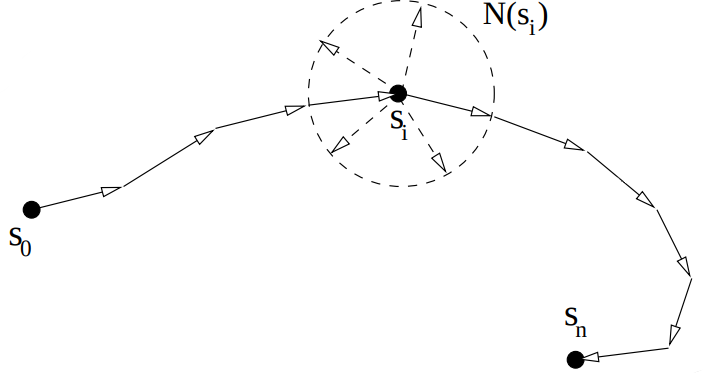
\includegraphics[width=0.55\textwidth]{./figs/local_search.png}
  \end{figure}
\end{frame}